\section{Метод конечных разностей во временной области}

Метод конечных разностей во временной области относится к общему классу сеточных методов решения дифференциальных уравнений. В его рамках уравнения Максвелла подвергаются дискретизации с использованием центрально-разностной аппроксимации как по временной, так и по пространственным координатам. Полученные конечно-разностные уравнения решаются программными или аппаратными средствами в каждой точке временной сетки, причём компоненты вектора напряжённости магнитного поля смещены на половину шага дискретизации относительно компонент вектора напряженности электрического поля вдоль каждой оси. Расчёт полей в ячейках сетки повторяется до тех пор, пока не будет получено решение поставленной задачи в интересующем промежутке времени.

% Базовый алгоритм FDTD; сосредоточенный резистивный источник напряжения; PML

Существует также большое количество расширений метода, наиболее популярным из которых являются разнообразные поглощающие граничные условия, преобразование ближнего поля в дальнее, моделирование сосредоточенных активных и пассивных элементов. В данной работе были реализованы только базовый алгоритм FDTD, сосредоточенный резистивный источник напряжения и поглощающие граничные условия PML.

\subsection{Принципы работы метода}

Рассмотрим систему из четырёх векторных уравнений Максвелла, записанных в системе единиц СИ:
\begin{equation}
    \label{eq:MaxwellEquations}
	\begin{cases}
		\Rot\vec{E} = \sigma_{H}\vec{H}-\parder{\vec{B}}{t}, \\
		\Rot\vec{H} = \sigma_{E}\vec{E}+\parder{\vec{D}}{t}, \\
		\Div\vec{D} = \rho, \\
		\Div\vec{B} = 0.
	\end{cases}
\end{equation}

В системе~\eqref{eq:MaxwellEquations} использованы следующие обозначения:
\begin{itemize}
\item $ \vec{E} $ --- напряжённость электрического поля,
\item $ \vec{H} $ --- напряжённость магнитного поля,
\item $ \vec{B} $ --- магнитная индукция ($ \vec{B} = \mu\mu_{0}\vec{H} $),
\item $ \vec{D} $ --- электрическая индукция ($ \vec{D} = \varepsilon\varepsilon_{0}\vec{E} $),
\item $ \varepsilon $ --- относительная диэлектрическая проницаемость,
\item $ \mu $ --- относительная магнитная проницаемость,
\item $ \sigma_{E} $ --- удельная электрическая проводимость,
\item $ \sigma_{H} $ --- удельная магнитная проводимость,
\item $ \rho $ --- плотность стороннего электрического заряда,
\item $ \varepsilon_{0} $ --- электрическая постоянная ($ \varepsilon_{0} \approx 8,8542 $ $\text Ф/\text м$),
\item $ \mu_{0} $ --- магнитная постоянная ($ \mu_{0}= 4\pi \cdot 10^{-7} $ $\text {Гн}/\text м$). \\
\end{itemize}

Рассматривая уравнения Максвелла, можно заметить, что изменение значения вектора индукции электрического поля во времени (частная производная вектора $ \vec{D} $ по времени) зависит от изменения магнитного поля в пространстве (ротор вектора $ \vec{H} $). Поэтому значение вектора электрического поля в каждой точке пространства в определённый момент времени будет зависеть от значения этого же вектора в предыдущий момент времени и от изменения распределения вектора напряжённости магнитного поля в пространстве. Аналогичным образом значение вектора $ \vec{H} $ в определённой точке и в определённый момент времени зависит от своего значения в предыдущий момент времени и от изменения распределения вектора $ \vec{E} $  в пространстве.

Исходя из этих требований, на время выполнения каждой итерации алгоритма нам необходимо хранить в памяти компьютера значения векторов $ \vec{E} $ и $ \vec{H} $ в предыдущий момент времени. Под \textit{итерацией} здесь и далее подразумевается расчёт значения вектора $ \vec{E} $ или $ \vec{H} $ в определённой точке в определённый момент времени.

Расчёт трёхмерных электромагнитных структур сильно усложняет вычисление ротора полей. В связи с этим американским математиком китайского происхождения Кейном И была разработана схема расчёта, в которой электрическая и магнитная сетки сдвинуты относительно друг друга так, что магнитное поле по каждой оси рассчитывается в точках, расположенных ровно между точками, в которых рассчитывается электрическое поле, и наоборот. Эта схема сейчас известна как \textit{сетка И}. Её графическая модель представлена на рис.~\ref{fig:YeeGrid}.

%% --
\begin{figure}[p]
\centering
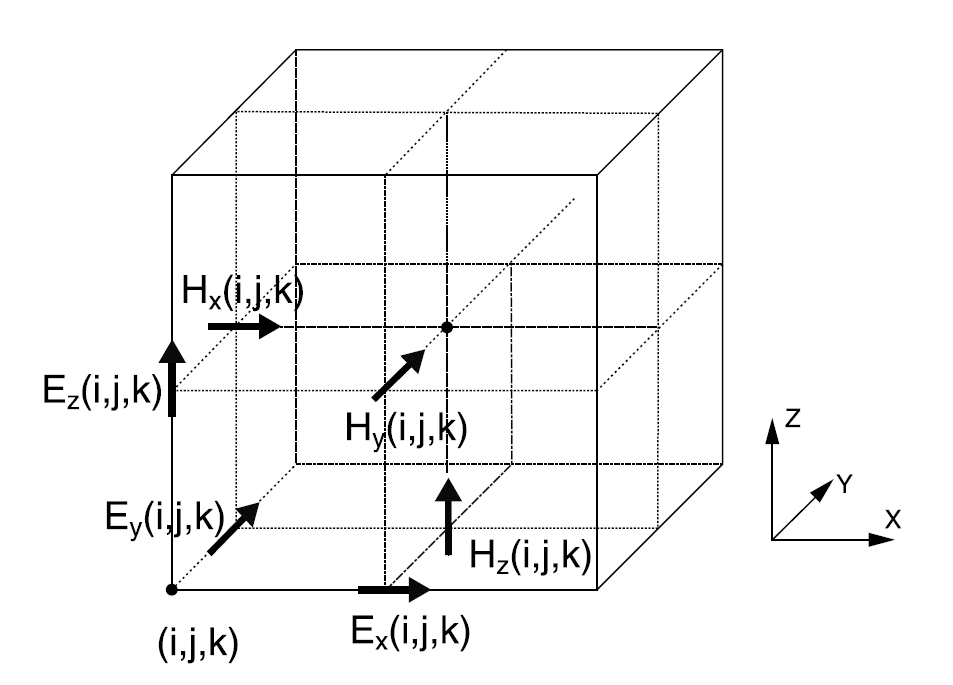
\includegraphics[width=1\textwidth]{include/graphics/image1}
\caption{Поля в ячейке сетки И.}
\label{fig:YeeGrid}
\end{figure}

\subsection{Входные параметры задачи}

На практике для численного решения какой-либо задачи электродинамики необходимо задать счётный объём. \textit{Счётный объём} (или \textit{счётная область}) --- это та область пространства, в пределах которой выполняется численное моделирование, и осуществляется непосредственный расчёт электромагнитных полей.

Счётная область разбивается на ячейки при помощи сетки И; в каждом узле сетки задаются значения электрических и магнитных проницаемостей и проводимостей. Чаще всего в качестве базового материала счётного объёма рассматривают вакуум (или воздух), в отдельных узлах сетки помещаются металлические или диэлектрические структуры. Тем не менее, алгоритм вполне позволяет задать произвольные значения вышеперечисленных величин для каждой точки объёма.

Кроме того, для моделирования реальных задач необходимы источники поля: некоторая структура, способная создавать электромагнитное возмущение внутри счётного объёма. Так, среди прочего, FDTD позволяет симулировать возбуждение электромагнитных колебаний при помощи падающей электромагнитной волны или точечного источника напряжения.

\subsection{Особенности метода}

Отличительной особенностью метода конечных разностей во временной области является его относительная простота. К достоинствам метода также можно отнести возможность создавать анимированные изображения распространения волновых процессов в счётном объеме, что может быть очень полезно для понимания происходящих в модели процессов и позволяет удостовериться в её корректности.

Основной недостаток метода --- обязательность разбиения счётного объёма на ячейки сетки И, причём величина шага дискретизации по пространственным координатам должна быть достаточно малой по сравнению с наименьшей длиной волны, встречающейся в конкретной задаче. Кроме того, эта величина ограничивает детализацию распределения материалов в пространстве, поэтому может оказаться, что счётный объём должен быть разделен на очень большое число ячеек, что влечёт за собой большие затраты памяти и увеличивает время моделирования.

Ещё одним недостатком FDTD является обязательность вычисления параметров поля в каждой точке счётного объёма. Так, при необходимости найти поле на некотором отдалении от источника придётся производить расчёт во всех точках, что находятся между источником и интересующей точкой.

К тому же, счётная область обязательно должна быть конечной. В большинстве случаев это достигается использованием искусственных граничных условий, но они, как правило, вызывают дополнительные искажения.

\subsection{Базовые уравнения}

% TODO: Add reference to `Computational Electrodynamics'

Как уже было сказано, метод FDTD предполагает введение сетки, которая в простейшем случае представляет собой обыкновенный трёхмерный массив, в котором хранятся векторы полей и пространственная структура. Процедура расчёта заключается в поочерёдном обращении всех элементов этого массива в порядке возрастания индексов и последующем перевычислении его элементов по приведенным ниже формулам.

Выражения для компонент магнитного поля:
\label{eq:BaseFdtdEquations}
\begin{align*}
	\Yee{H_x}{n+1/2}{i,j,k} &=
        \Yee{H_x}{n-1/2}{i,j,k} - \frac{\frac{\Delta{t}}{\mu}}
             {1+\frac{\sigma_H\Delta{t}}{2\mu}}
        \left[
            \frac{\yee{E_z}{n}{i,j+1,k} - \yee{E_z}{n}{i,j,k}}{\Delta{y}} -
            \frac{\yee{E_y}{n}{i,j,k+1} - \yee{E_y}{n}{i,j,k}}{\Delta{z}}
        \right], \\
	\Yee{H_y}{n+1/2}{i,j,k} &=
        \Yee{H_y}{n-1/2}{i,j,k} - \frac{\frac{\Delta{t}}{\mu}}
             {1+\frac{\sigma_H\Delta{t}}{2\mu}}
        \left[
            \frac{\yee{E_x}{n}{i,j,k+1} - \yee{E_x}{n}{i,j,k}}{\Delta{z}} -
            \frac{\yee{E_z}{n}{i+1,j,k} - \yee{E_z}{n}{i,j,k}}{\Delta{x}}
        \right], \\
	\Yee{H_z}{n+1/2}{i,j,k} &=
        \Yee{H_z}{n-1/2}{i,j,k} - \frac{\frac{\Delta{t}}{\mu}}
             {1+\frac{\sigma_H\Delta{t}}{2\mu}}
        \left[
            \frac{\yee{E_y}{n}{i+1,j,k} - \yee{E_y}{n}{i,j,k}}{\Delta{x}} -
            \frac{\yee{E_x}{n}{i,j+1,k} - \yee{E_x}{n}{i,j,k}}{\Delta{y}}
        \right],
\end{align*}

Выражения для компонент электрического поля:
\begin{align*}
	\fYee{E_x}{n+1}{i,j,k} &=
        \frac{1-\frac{\sigma_E\Delta{t}}{2\varepsilon}}
             {1+\frac{\sigma_E\Delta{t}}{2\varepsilon}} \fYee{E_x}{n}{i,j,k} +
        \frac{\frac{\Delta{t}}{\varepsilon}}
             {1+\frac{\sigma_E\Delta{t}}{2\varepsilon}}
        \left[
            \frac{\yee{H_z}{n+1/2}{i,j,k} - \yee{H_z}{n+1/2}{i,j-1,k}}{\Delta{y}} -
            \frac{\yee{H_y}{n+1/2}{i,j,k} - \yee{H_y}{n+1/2}{i,j,k-1}}{\Delta{z}}
        \right], \\
	\fYee{E_y}{n+1}{i,j,k} &=
        \frac{1-\frac{\sigma_E\Delta{t}}{2\varepsilon}}
	         {1+\frac{\sigma_E\Delta{t}}{2\varepsilon}} \fYee{E_y}{n}{i,j,k} +
        \frac{\frac{\Delta{t}}{\varepsilon}}
             {1+\frac{\sigma_E\Delta{t}}{2\varepsilon}}
        \left[
            \frac{\yee{H_x}{n+1/2}{i,j,k} - \yee{H_x}{n+1/2}{i,j,k-1}}{\Delta{z}} -
            \frac{\yee{H_z}{n+1/2}{i,j,k} - \yee{H_z}{n+1/2}{i-1,j,k}}{\Delta{x}}
        \right], \\
	\fYee{E_z}{n+1}{i,j,k} &=
        \frac{1-\frac{\sigma_E\Delta{t}}{2\varepsilon}}
             {1+\frac{\sigma_E\Delta{t}}{2\varepsilon}} \fYee{E_z}{n}{i,j,k} +
        \frac{\frac{\Delta{t}}{\varepsilon}}
             {1+\frac{\sigma_E\Delta{t}}{2\varepsilon}}
        \left[
            \frac{\yee{H_y}{n+1/2}{i,j,k} - \yee{H_y}{n+1/2}{i-1,j,k}}{\Delta{x}} -
            \frac{\yee{H_x}{n+1/2}{i,j,k} - \yee{H_x}{n+1/2}{i,j-1,k}}{\Delta{y}}
        \right].
\end{align*}

Выше приведены формулы, позволяющие вычислить каждую из компонент векторов напряжённости электрического и магнитного полей. В этих формулах используются следующие обозначения:
\begin{itemize}
\item $ \sigma_E $ --- удельная электрическая проводимость материала в ячейке сетки;
\item $ \sigma_H $ --- удельная магнитная проводимость материала в ячейке сетки;
\item $ \varepsilon $ --- абсолютная диэлектрическая проницаемость материала;
\item $ \mu $ --- абсолютная магнитная проницаемость материала;
\item $ \Delta{t} $ --- шаг дискретизации по времени;
\item $ \Delta{x} $, $ \Delta{y} $, $ \Delta{z} $ --- шаги дискретизации по пространственным координатам. \\
\end{itemize}

Необходимо заметить, что величина $ \Delta{t} $ определяет частотные характеристики метода: наивысшая частота в спектре сигналов, распространение которых моделируется, не должна превышать $ f_{max} = \frac{1}{\Delta{t}} $.

Также величина $ \Delta{t} $ должна удовлетворять условию Куранта:
\begin{align*}
\Delta{t} < \frac{1}{c\sqrt{\frac{1}{\Delta{x}^2} + \frac{1}{\Delta{y}^2} + \frac{1}{\Delta{z}^2}}}
\end{align*}

% TODO: Replace quotation mark

Пересчёт значений компонент выполняется «на месте», то есть рассчитанное в каждый последующий момент времени значение помещается в ту же ячейку сетки И, в которой находилось значение для предыдущего момента. Это позволяет несколько снизить требования к оперативной памяти, предъявляемые методом.

\subsection{Точечный резистивный источник}

Возможность моделировать сосредоточенные элементы вводится дополнительно, при этом границы применения метода существенно расширяются. В частности, точечный генератор напряжения с заданным внутренним сопротивлением оказывается весьма удобной моделью источника питания.

Достоинством этого дополнения FDTD является то, что вид уравнений меняется весьма незначительно. Если источник ориентирован вдоль оси $Z$, то в системе уравнений Максвелла~\eqref{eq:MaxwellEquations} изменится только одна составляющая векторного уравнения для ротора вектора магнитной напряжённости:

\begin{equation}
    \label{eq:LumpedSource:MaxwellEquationsAmendment}
    (\Rot\vec{H})_z = \varepsilon\frac{\partial{E_z}}{\partial{t}} +
        \sigma E_z + \frac{I_L}{\Delta{x}\Delta{y}},
\end{equation}
где $ I_L $ --- ток через источник.

Подвергнув уравнение~\eqref{eq:LumpedSource:MaxwellEquationsAmendment} действию конечно-разностной схемы и положив~$\sigma_E=0$, получим следующую формулу:
\begin{multline}
    \label{eq:LumpedSource:FdtdEquationsAmendmentWithI}
    \fYee{E_z}{n+1}{i,j,k} = \fYee{E_z}{n}{i,j,k} +
        \frac{\Delta{t}}{\yee{\varepsilon}{}{i,j,k}}
        \left[
            \frac{\yee{H_y}{n+1}{i,j,k}-\yee{H_y}{n+1}{i-1,j,k}}{\Delta{x}} -
            \frac{\yee{H_x}{n+1}{i,j,k}-\yee{H_x}{n+1}{i,j-1,k}}{\Delta{y}}
        \right] - \\ -
        \frac{\yee{I_L}{n+1}{}\Delta{t}}
             {\yee{\varepsilon}{}{i,j,k}\Delta{x}\Delta{y}}.
\end{multline}

Согласно закону Ома, для рассматриваемого сосредоточенного генератора напряжения
с внутренним сопротивлением $R$ будет иметь место равенство
\begin{equation}
    \label{eq:LumpedSource:OhmLaw}
    \fYee{I_L}{n+1}{} = \frac{\Delta{z}}{2R}
    \left(
        \fYee{E_z}{n+1}{i,j,k} - \Yee{E_z}{n}{i,j,k}
    \right) +
    \frac{\yee{U_s}{n+1}{}}{R},
\end{equation}
где $U_s$ --- генерируемое источником напряжение.

После подстановки~\eqref{eq:LumpedSource:OhmLaw}
в~\eqref{eq:LumpedSource:FdtdEquationsAmendmentWithI} получим простое уравнение
для~$E_z$:
\begin{multline*}
    \label{eq:LumpedSource:FdtdEquationsAmendmentWithU}
    \fYee{E_z}{n+1}{i,j,k} =
        \fYee{C_E}{}{i,j,k}\fYee{E_z}{n}{i,j,k}~~+~~
        \Yee{C_H}{}{i,j,k}
        \left[
            \frac{\yee{H_y}{n+1}{i,j,k}-\yee{H_y}{n+1}{i-1,j,k}}{\Delta{x}}
        \right. - \\ -
        \left.
            \frac{\yee{H_x}{n+1}{i,j,k}-\yee{H_x}{n+1}{i,j-1,k}}{\Delta{y}} +
            \frac{\yee{U_s}{n+1}{}}{R\Delta{x}\Delta{y}}
        \right],
\end{multline*}
где $C_E$ и~$C_H$ определяются по следующим формулам:
\begin{equation*}
    \newcommand\XA{\displaystyle
        \frac{\Delta{t}}{\yee{\varepsilon}{}{i,j,k}}}
    \newcommand\XB{\displaystyle
        \frac{\Delta{t}\Delta{z}}{2R\yee{\varepsilon}{}{i,j,k}\Delta{x}\Delta{y}}}
    % --
    \fYee{C_E}{}{i,j,k} = \frac{1-\XB}{1+\XB}, \quad
    \fYee{C_H}{}{i,j,k} = \frac{\XA}{1+\XB}.
\end{equation*}

Формулы для прочих компонент остаются неизменными.

\clearpage